\chapter{Literature Review}
\section{Genre detection in songs}
Nanni et al. (2018)\cite{nanni_ensemble_2018} investigated the effectiveness of acoustic features versus visual features in music genre detection in their paper Musical genre classification of audio signals. They observed that the features attained by classical methods and the features used by CNN contain different information. By combining the features obtained, they acquired more successful results than previous studies.

Ceylan et al. (2021)\cite{ceylan_automatic_2021} investigated the use of MFCC graphs in music genre detection in their paper Ensemble of deep learning, visual and acoustic features for music genre classification. Music segments from the GTZAN dataset of length 3  seconds were converted into MFCC graphs using python’s librosa library and passed as input into a convolutional neural network. They obtained accuracy comparable to or higher than other studies in which many features or more complex and combined deep learning models were used. 

\section{Emotional models}

The emotional models are classified into 2 major classes as can be seen in Figure \ref{fig: emotional models} one model is categorical and the other is dimensional model \cite{emotion_models}

\subsection{Categorical model}
Emotions are recognized with the help of words denoting emotions or class tags.
The categorical model either makes use of six basic emotion classes namely anger, disgust, fear, joy, sadness, and surprise or uses domain-specific expressive classes such as boredom, confusion. There are both significant and unrelated
emotions in this model. Each emotion has a specific set of features that express provoking circumstances or
reactions. Most research in affective computing has concentrated on the aforementioned six basic emotions
 
 
 
\subsection{Dimensional model}
DImensional model denotes effects in a dimensional form. A common set of dimensions link the various emotional states in this model. They are defined in a
two(valence and arousal) or three ( valence, arousal, and power) dimensional space. Each emotion occupies a position in this space. The valence dimension defines the positivity or negativity of emotion and ranges from unpleasant feelings to pleasant feelings (sense of happiness). The arousal dimension denotes the level of excitement that the emotion depicts, and it ranges from sleepiness or boredom to wild excitement. The influence dimension denotes the degree of power such as a sense of control over the emotion.

\begin{figure}[H]
\centering
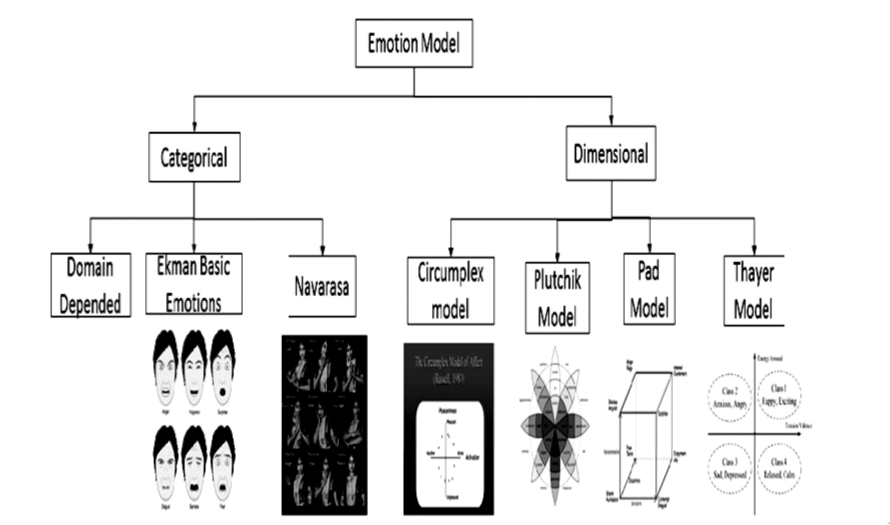
\includegraphics[width=\textwidth]{imgs/emotion_models.png}
\caption{Emotional Models}
\label{fig: emotional models}
\end{figure}

\section{Plutchik emotional model}
Plutchik \cite{plutchik_emotions} states that there are eight basic emotions: 
\begin{enumerate}
	\item Joy
	\item Trust
	\item Fear
	\item Surprise
	\item Sadness
	\item Anticipation
	\item Anger
	\item Disgust
\end{enumerate}
Plutchik created the wheel of emotions as can be seen in Figure \ref{fig: plutchik model}, which illustrates the various relationships among the emotions. \newline

Each primary emotion also has a polar opposite, so that:
\begin{itemize}
	\item Joy is the opposite of sadness.
	\item Fear is the opposite of anger.
	\item Anticipation is the opposite of surprise.
	\item Disgust is the opposite of trust.
\end{itemize}


\begin{figure}[H]
\centering
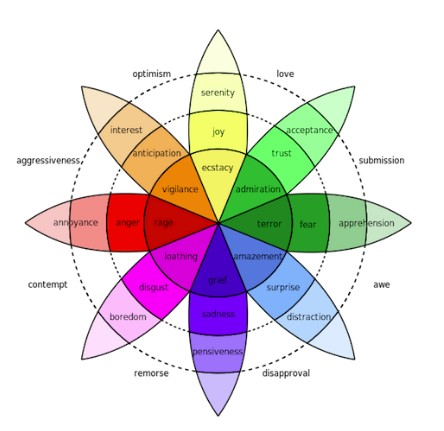
\includegraphics[width=\textwidth]{imgs/plutchik_model.jpg}
\caption{Plutchik's Emotional Model}
\label{fig: plutchik model}
\end{figure}


\section{Web Scraping}
Web scraping, also known as web extraction or harvesting, is a technique to extract data from the World Wide Web and save it to a file system or database for later retrieval or analysis\cite{webscraping}\newline

Web scraping is accomplished either manually by a user or automatically by a bot or web crawler. Due to the fact that an enormous amount of heterogeneous data is constantly generated on the World Wide Web.\newline

To adapt to a variety of scenarios, current web scraping techniques have become customized from smaller ad hoc, human-aided procedures to the utilization of fully automated systems that are able to convert entire websites into well-organized datasets, and are often performed using automated tools.
\section{Mel Scale}
The Mel scale is a fundamental result of psychoacous tics, relating real frequency to perceived frequency. The foundation of the mel scale is the classic work of Stevens and Volkman\cite{mel-scale}. Their results and variations thereof appear in almost every speech book. In this paper we address certain issues regarding the Mel scale and in particlar we discuss the issue of fitting the Mel scale and the implications and physical meaning of the fitting formula. Many authors have attempted fit ting formulas for a variety of reasons. Most important among these is that such fits sometimes give an indi cation of the underlying physical phenomenon. Furthermore, such fits may be used to develop models for the psychoacoustic scale. \newline

An alternate definition of the mel scale is that it is a quasi-logarithmic function of acoustic frequency designed such that perceptually similar pitch intervals (e.g. octaves) appear equal in width over the full hearing range.

\section{MFCC}
Mel Frequency Cepstrum or MFC is a representation of the short-term power spectrum of a sound, which is based on a linear cosine transform of a log power spectrum on a nonlinear mel scale of frequency. A visualization of an MFCC can be seen in Figure \ref{fig: mfcc}
Mel Frequency Cepstrum Coefficients or MFCC are the coefficients that make up the MFC representation  \cite{mel-frequency_2021} \newline

Standard MFCC computation technique utilizes discrete cosine transform (DCT) for decorrelating log energies of filter bank output. The use of DCT is reasonable here as the covariance matrix of Mel filter bank log energy or MFLE can be compared with that of highly correlated Markov-I process.\cite{mfcc_speaker_2012}

\begin{figure}[H]
\centering
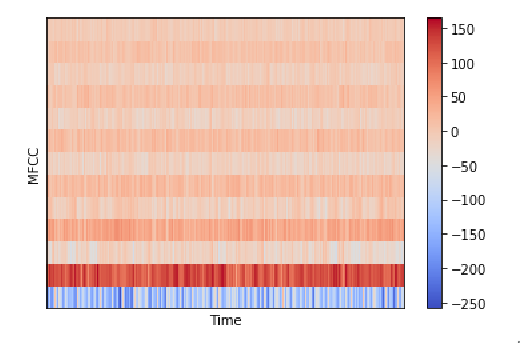
\includegraphics[width=\textwidth]{imgs/mfcc.png}
\caption{MFCC spectrum}
\label{fig: mfcc}
\end{figure}


\section{Existing corpora for emotion classification in text}
Bostan and Klinger (2018) \cite{emotion_classification_datasets}, performed an analysis on existing corpora for emotion classification in text. They analyzed 14 existing emotion datasets, nearly all of which use an annotation scheme based on Ekman (Ekman, 1969 \cite{ekman_pan-cultural_1969}) with many adding a few labels often following Plutchik’s theory of emotions (Plutchik, 1980 \cite{plutchik_emotions})


\section{The GTZAN dataset}
Tzanetakis and Cook (2002)\cite{tzanetakis_musical_2002}  investigated automatically classifying audio signals into a hierarchy of musical genres namely:

\begin{itemize}
	\item Classical
	\item Country
	\item Disco
	\item Hiphop
	\item Jazz
	\item Rock
	\item Blues
	\item Reggae
	\item Pop
	\item Metal
\end{itemize}

These researchers made use of several musical features such as rhythm, timbre, and pitch in the process of classifying music. They also produced the most widely used dataset for music genre detection, the GTZAN dataset \cite{gtzan_dataset}

\section{XED dataset}
The XED dataset was produced by Ohman et. al. \cite{ohman-etal-2020-xed}. The XED dataset uses Plutchik’s core emotions as its annotation scheme resulting in 8 distinct emotion categories plus neutral. The dataset uses the OPUS (Lison and Tiedemann, 2016 \cite{opensubtitles2016}) parallel movie subtitle corpus of subtitles collected from opensubtitles.org \newline

The dataset consists of tab separated files(tsv) mapping lines from the subtitles to emotions from Plutchik’s model.

\section{Convolutional Neural Network}
Convolutional neural networks are distinguished from other neural networks by their superior performance with image, speech, or audio signal inputs. They have three main types of layers, which are:
\begin{itemize}
	\item Convolutional layer
	\item Pooling layer
	\item Fully-connected (FC) layer
\end{itemize}

The convolutional layer is the first layer of a convolutional network. While convolutional layers can be followed by additional convolutional layers or pooling layers, the fully-connected layer is the final layer. With each layer, the CNN increases in its complexity, identifying greater portions of the image. Earlier layers focus on simple features, such as colors and edges. As the image data progresses through the layers of the CNN, it starts to recognize larger elements or shapes of the object until it finally identifies the intended object.\newline

The convolutional layer is the core building block of a CNN, and it is where the majority of computation occurs. An illustration of this computation is shown in Figure \ref{fig: cnn}. It requires a few components, which are input data, a filter, and a feature map. Let’s assume that the input will be a color image, which is made up of a matrix of pixels in 3D. This means that the input will have three dimensions—a height, width, and depth—which correspond to RGB in an image. We also have a feature detector, also known as a kernel or a filter, which will move across the receptive fields of the image, checking if the feature is present. This process is known as a convolution.

\begin{figure}[H]
\centering
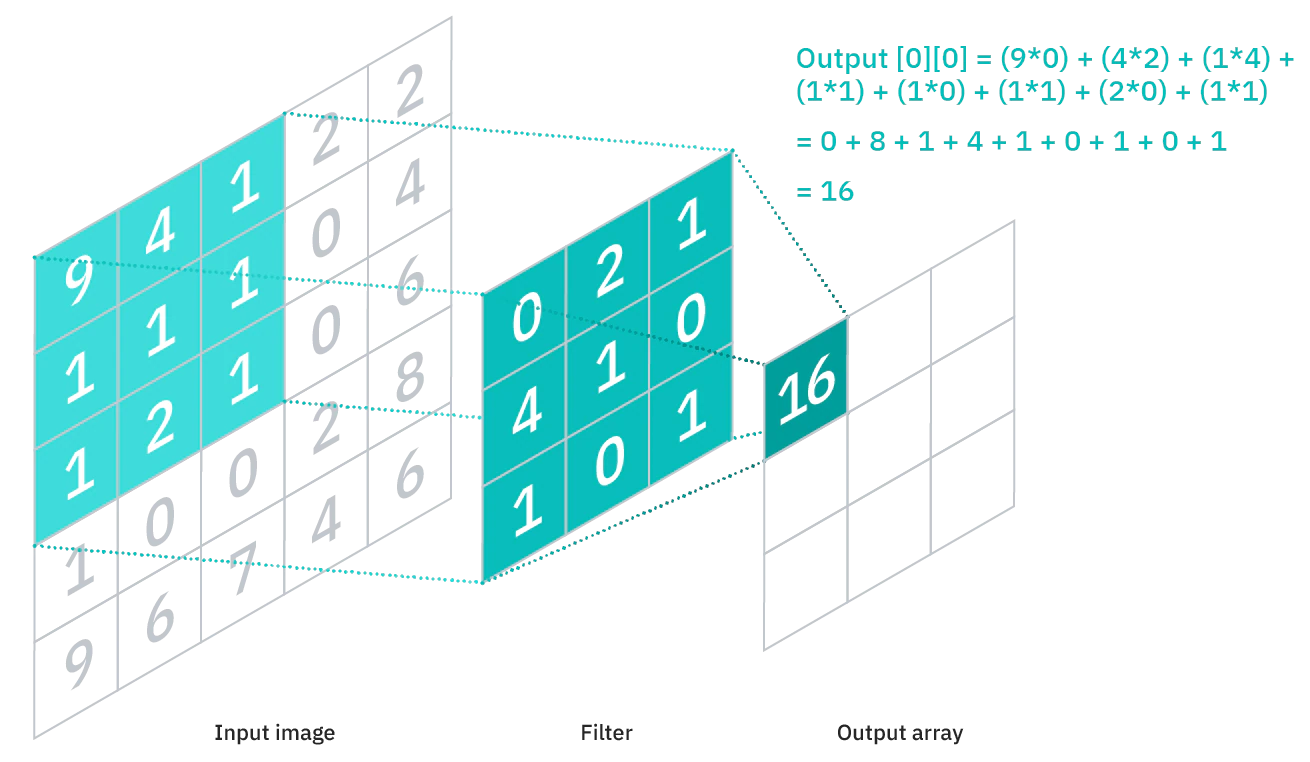
\includegraphics[width=\textwidth]{imgs/cnn.png}
\caption{Working of a Convolutional Neural Network}
\label{fig: cnn}
\end{figure}
\section{Recurrent Neural Network}
A recurrent neural network (RNN) is a type of artificial neural network which uses sequential data or time series data. These deep learning algorithms are commonly used for ordinal or temporal problems, such as language translation, natural language processing (nlp), speech recognition, and image captioning; they are incorporated into popular applications such as Siri, voice search, and Google Translate. Like feedforward and convolutional neural networks (CNNs), recurrent neural networks utilize training data to learn. They are distinguished by their "memory" as they take information from prior inputs to influence the current input and output. While traditional deep neural networks assume that inputs and outputs are independent of each other, the output of recurrent neural networks depend on the prior elements within the sequence as can be seen in Figure \ref{fig: rnn}. While future events would also be helpful in determining the output of a given sequence, unidirectional recurrent neural networks cannot account for these events in their predictions.

\begin{figure}[H]
\centering
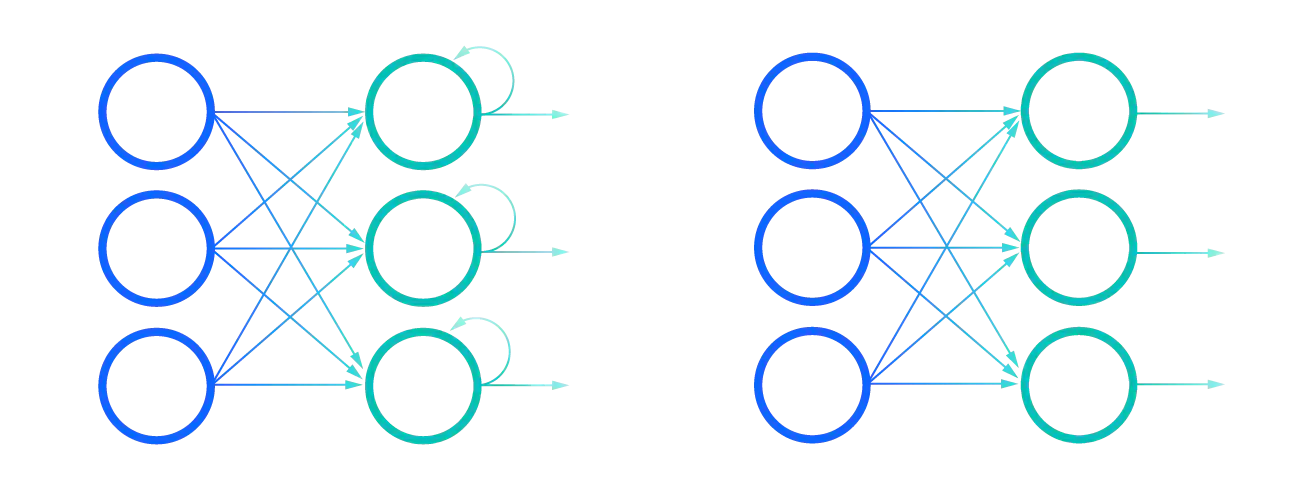
\includegraphics[width=\textwidth]{imgs/rnn.png}
\caption{Recurrent Neural Network vs. Feedforward Neural Network }
\label{fig: rnn}
\end{figure}
\section{Transfer Learning}
The reuse of a pre-trained model on a new problem is known as transfer learning in machine learning \cite{transfer_learning}. A machine uses the knowledge learned from a prior assignment to increase prediction about a new task in transfer learning. The knowledge of an already trained machine learning model is transferred to a different but closely linked problem throughout transfer learning as illustrated in \ref{fig: transferLearning}. For example, if you trained a simple classifier to predict whether an image contains a backpack, you could use the model’s training knowledge to identify other objects such as sunglasses. \newline

In computer vision, neural networks typically aim to detect edges in the first layer, forms in the middle layer, and task-specific features in the latter layers. The early and central layers are employed in transfer learning, and the latter layers are only retrained. It makes use of the labelled data from the task it was trained on.

\begin{figure}[H]
\centering
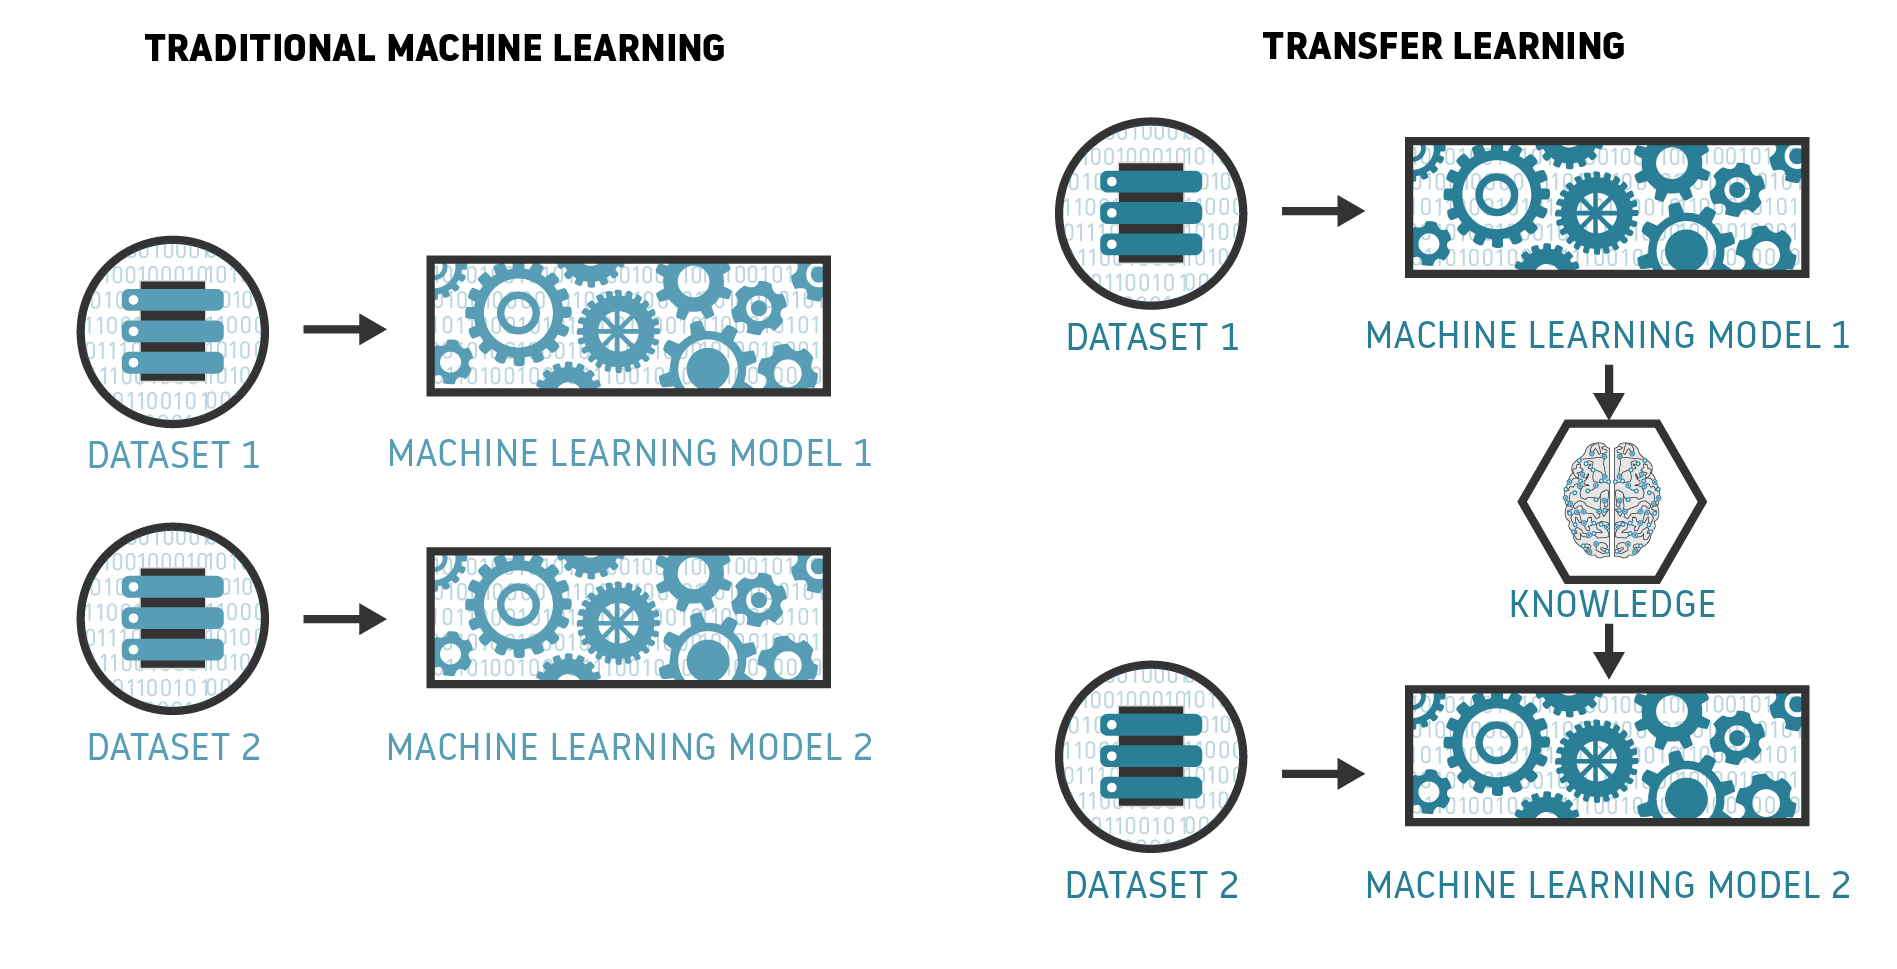
\includegraphics[width=\textwidth]{imgs/transferlearning.jpg}
\caption{Transfer Learning}
\label{fig: transferLearning}
\end{figure}

